\documentclass[12pt, letterpaper]{article}
\usepackage[titletoc,title]{appendix}
\usepackage{color}
\usepackage{booktabs}
\usepackage[usenames,dvipsnames,svgnames,table]{xcolor}
\definecolor{dark-red}{rgb}{0.75,0.10,0.10}
\definecolor{dark-blue}{rgb}{0.1,0.1,0.8}
\usepackage[margin=1in]{geometry}
\usepackage[linkcolor=dark-red,
			colorlinks=true,
			urlcolor=blue,
			pdfstartview={XYZ null null 1.00},
			pdfpagemode=UseNone,
			citecolor={dark-blue},
			pdftitle={Strength in Numbers}]{hyperref}
%\usepackage{biblatex}
\usepackage[utf8,latin1]{inputenc}
\usepackage{longtable}

\usepackage[multiple]{footmisc}

\usepackage{url}
\usepackage{setspace}
\usepackage{indentfirst}


\usepackage{multibib}
\newcites{sec}{Other Sources}
\usepackage{geometry} % see geometry.pdf on how to lay out the page. There's lots.
\geometry{letterpaper}               % This is 8.5x11 paper. Options are a4paper or a5paper or other...

\usepackage{graphicx}                % Handles inclusion of major graphics formats and allows use of
\usepackage{amsfonts,amssymb,amsbsy}
\usepackage{amsxtra}

\usepackage{natbib}

\usepackage{verbatim}

\setcitestyle{round,semicolon,aysep={},yysep={;}}

\usepackage{setspace}		     % Permits line spacing control. Options are \doublespacing, \onehalfspace
\usepackage{sectsty}		     % Permits control of section header styles
\usepackage{lscape}

\usepackage{fullpage}		%1-inch margins
\usepackage{multirow}
\usepackage{rotating}
\setlength{\parindent}{3em}

\usepackage[T1]{fontenc}
\usepackage{bm}
\usepackage{libertine}

\usepackage{chngcntr}

% tt font issues
% \renewcommand*{\ttdefault}{qcr}
\renewcommand{\ttdefault}{pcr}

\DeclareMathOperator*{\argmax}{arg\,max}

\usepackage{xr}
\externaldocument{../tabs/text/validation.tex}

\usepackage{lscape}
\renewcommand{\textfraction}{0}
\renewcommand{\topfraction}{0.95}
\renewcommand{\bottomfraction}{0.95}
\renewcommand{\floatpagefraction}{0.40}
\setcounter{totalnumber}{5}
\makeatletter
\providecommand\phantomcaption{\caption@refstepcounter\@captype}
\makeatother

\title{Strength in Numbers: Multiple Measures of \\Media Ideology\footnote{We thank Anjie Fang and Tony Hirst for scraping the Twitter data, and Matt Blackwell for offering useful comments.}}

\author{Gaurav Sood\thanks{Gaurav is a data scientist. He can be reached at: \href{mailto:gsood07@gmail.com}{\texttt{gsood07@gmail.com}}.} \and Philip Habel\thanks{Philip Habel is Senior Lecturer in Politics at the School of Social and Political Sciences at the University of Glasgow. He can be reached at \href{mailto:philiphabel@gmail.com}{philiphabel@gmail.com}}.}

\begin{document}
\maketitle

\begin{center}
\vspace{1cm}\textbf{NB:} Work in progress. Please ask the authors before citing.\\\vspace{1cm}
\end{center}


\begin{comment}

setwd(paste0(basedir, "uk_media_ideology/ms/"))
tools::texi2dvi("multiple_measures.tex", pdf=TRUE, clean=TRUE)
setwd(basedir)

\end{comment}

\begin{abstract}

\noindent Attempts at quantifying media ideology have generally taken one of two routes. Scholars have either exploited the similarity between phrases used by the news media and the politicians, or they have exploited the differences in composition of the audiences. We forgo the conventional reliance on one set of cues. Instead, we pool both text and audience based measures to estimate the ideological location of a number of media sources in the UK. The UK presents an appropriate environment for carrying out our research given ideology of members of parliament cannot be simply gotten via voting records. We combine corpora of parliamentary speech and party manifestos with Twitter data to produce more reliable measures of news media ideology and insight into differences between the two metrics.
\end{abstract}

\newpage
\doublespacing

According to Edmund Burke, the news media's capacity to hold the ear of the public makes it an equal partner in a democracy, a veritable ``fourth estate'' \citep{carlyle2003heroes}.  If power is what makes the news media an equal shareholder, it is its independence, and how dutifully it fulfills its responsibility, that explains its contribution to the success of a democracy. If the media favors one party (or ideological position) over another, its capacity to hold the politicians accountable---by informing the public about the functioning of the government---is necessarily diminished \citep[see, for e.g.,][]{larcinese2011}. And if the media doesn't present information on all sides of an issue, or cover candidates and elected officials fairly, public opinion may skew toward suboptimal alternatives.

Such concerns have led to a large literature on the measurement and impact of various kinds of bias in the news media. Extant research suggests that the news media disproportionately focuses on `negative' news, for e.g., coverage of declines in stock market outstrips coverage of gains \citep{goetzmann2016crash}, that local news media fixates on violent crime ---share of local news' coverage devoted to violent crime is manifolds actual share of violent crime \citep{gross2006covering}, and that local news exhibits racial bias---some local news media outlets show black criminals at higher rates than at which they are arrested \citep{dixon2000overrepresentation}. Research also suggests that such biases influence people's voting and policy preferences \citep[see, for e.g.,]{gilens2009americans, gilliam2000prime}.

More recently, the rise in elite and mass polarization in the US and the UK \citep{mccarty2016polarized, iyengar2012} has led to an increase in accusations of partisan bias \citep{ladd2011}. And while accusations of bias can't always be taken at face value, given the ubiquity of `sidedness'-biases \citep{vallone1985hostile}, the depth of concern has been severe enough to foment inquiry. As a result, a growing literature attempts to measure media bias, and impact of consumption of biased media on voting decisions, policy opinions, and representation \citep[see, for e.g.,][]{groseclose2005, gentzkow2010, dellavigna2007}. The literature has taken greater urgency post studies suggesting that biased media can have a tangible impact on vote shares \citep{dellavigna2007, martin2014}.

Hitherto, most of the attempts at measuring partisan bias have fallen into two camps. The first assumes that elected officials hold ideological positions, and that their voting records and speech reveal these positions. Armed with the speech of members of Congress, scholars turned to news sources to examine the similarity of their communication to that of politicians. If Republicans, for example, use the phrase `death tax' instead of `estate tax' more than say Democrats, we learn something about the ideology of a news media outlet that exhibits the same pattern \citep[e.g.,][]{gentzkow2010,groseclose2005}.

A second camp uses audience composition to understand bias. The assumption here is that a more liberal (conservative) audience will gravitate toward more liberal (conservative) news sources. Early work in this area was based principally on survey evidence, with respondents being asked questions about their own ideology and then the frequency at which they watch news channels or programs \citep[see][for a recent example]{stroud2011}. More recently, scholars have taken advantage of behavioral measures, including patterns of following media outlets on social media. If a news outlet attracts liberal (conservative) followers, then one can estimate media slant, and order the ideology of news outlets accordingly \citep{gentzkow2011, barbera2016}.

In this paper, we forgo the typical strategy of using just one source of information, and instead rely on multiple sources. We do so for two reasons: a) to build more reliable measures, b) to build more granular measures---measures by `topic.' We pool both text and audience based measures to estimate ideological location of a large set of media sources in the United Kingdom, an interesting and novel context for two reasons. The UK, with its particularly diverse and rich media environment, featuring both publicly funded and commercial media organization, numerous broadsheet publications, and tabloid presses, not to mention local media outlets, provides a great case study. And secondly, it is a country where politician's votes carry little ideological information beyond party due to whipping. We estimate the ideology of a large set of media sources using a large novel text corpora of UK news media---we have crawled more than 2 million pages---and data on Twitter followers of both politicians and media outlets. We present insights into how slant of news sources relates to audiences in the UK.

\section*{Assessing Media Ideology}

Accusations of political slant against the news media are common. And some scholars have exploited these perceptions of bias to measure the ideology of news media \citep{dilliplane2011all, dilliplane2014activation}. Perceptions, however, do not always capture reality, particularly where media bias is concerned. A great deal of research shows that people tend to evaluate the credibility and evenhandedness of a piece of information based on whether or not it is congenial to their prior attitudes---rating uncongenial information as less reliable and more skewed than congenial information \citep[see, for e.g.,][]{vallone1985hostile, lord1979biased, khanna2015}. Unsurprisingly, thus, a large share of the variation in ratings of news media ideology is explained by rater's partisanship \citep{sood2016}.

Given the problems with the use of perceptions of media organizations' ideology, many scholars have forgone them. Instead, some rely on exploiting the audience composition. The theory goes that in a free capitalist media system, people's choices reflect their preferences. Thus, based on self-reports of what news media people consume, we could use the proportion of audience of a media outlet that is Republican as an indicator of its ideology. But serious concerns remain about reported consumption---people tend to greatly overstate the extent to which they watch both partisan and non-partisan news \citep{prior2013media}. In lieu of these concerns, some scholars derive audience metrics from passive observation of media consumption \citep{flaxman2014}.

But even if we have a perfect measure of the audience, we cannot simply assume a one-to-one relationship between audience' partisanship (or ideology) and their choice to consume news from a particular outlet. The relation between viewership and preferences is complex \citep{sood2016}. For instance, people's viewing behavior can be affected by small changes in convenience \citep{martin2014}. To address this particular critique, others have used more complex structural models linking behavior to preferences (and ideological locations) \citep{gentzkow2011, barbera2016}.

The basic structural model linking news media choices to ideological preferences includes a utility function that is sensitive to the distance between the news media and person's ideology. Such a structural model has some grounding in psychology. People like to consume ideologically congenial information because there are psychological costs to consuming messages uncongenial to their existing political beliefs \citet{festinger1957}. Typically, the loss to utility as a result of consuming information different from the ideal point is taken to be quadratic \citep[see, for e.g.,][]{gentzkow2011}. \citet{barbera2015} and \citet{barbera2016} add to this standard model in three ways: a) limit the data to politically interested people---people whose news media consumption is more sensitive to ideology \citep{iyengar2009}, b) validate the model and the choice of the subset using a training set (Congress) for which the ideology is known, and c) allow for fixed effects and other covariates, like location, number of subscribers, etc. to regress out other reasons why someone may subscribe to a news outlet. We opt for this particular strategy as one of the ways to measure ideology of the news media in the UK.

Estimating ideology based on audience composition is but one way of measuring ideology of the news media. Another promising way is systematic analysis of text. To that end, others have exploited expressed opinions on issues---positions expressed by newspapers on editorial pages to scale or score them \citep{ho2008,puglisi2011,puglisi2015}. For example, \citep{habel2012} uses editorial positions by the \emph{New York Times} and \emph{Wall Street Journal} on the same votes used by the ADA to scale members of Congress over a 50 year period. Here the limitation is that the ideology of the editorial page may be quite distinct from bias in news coverage---for example, the New York Times is relatively moderate in its news coverage \citep{gentzkow2010} while offering a distinctly liberal voice on its editorial pages \citep{habel2012}---and editorial positions are both rare and self-selected.

To sidestep the issues with expressed positions, \citet{groseclose2005} devised an innovative indirect approach to measuring media bias. Members of Congress give speeches in Congress. And during these speeches, politicians reference think tanks. And some of the think tanks that are referenced have distinct ideological positions, measures of which can be readily obtained from the interest group, Americans for Democratic Action (ADA). \citet{groseclose2005} use these think tank citations to derive a relationship between think tank citations and ideology. And then use that relationship to impute ideology of media outlets, which also cite think tanks. Building on \citet{groseclose2005}, \citet{gentzkow2010} look at broader language use, and impute ideological scores for mass media accordingly. A closer inspection of some of the models suggests that while the models are very good at discriminating across parties, they are poor at discriminating within parties \citep{barbera2016, gentzkow2015measuring}. Additional challenges associated with these indirect methods include discriminating between slant and agendas \citep[see, for e.g.,][]{quinn2010}. However, we pool insights gleaned from these models with audience based models in an attempt to build more reliable and more granular estimates.

\section*{The British Context}

The UK has a liberal media system \citep{hallin2011comparing}. Like the US, the UK features a profit-oriented media with low levels of government regulation, and independence from political parties \citep{hallin2004}. Yet there are several features that distinguish it from the US. The UK is particularly well known for its subsidized and regulated broadcast outlet, the British Broadcasting Corporation (BBC), which is often the focus of both public concern and scholarly work investigating bias given the potential for government's role in influencing what is broadcast. Beyond the BBC, there exists a loosely regulated and profit-oriented broadcast and print media. The print outlets range from the widely respected broadsheets, such as \textit{The Telegraph} (associated with conservative views, referred to by its critics as ``The Torygraph"), \textit{The Guardian} (its putative liberal counterpart), \textit{The Times of London} (understood to be more middle of the road), to outlets carrying more soft news, such as \textit{The Daily Mail}, and \textit{The Sun}, the most widely circulated newspaper. Beyond national broadcast channels and presses, there are also regional ones---including, for example, counterparts with names such as \textit{Scottish Television} (STV) in contrast to the national \textit{Independent Television} (ITV), or \textit{The Scottish Sun} to \textit{The Sun}. Aside from these is an abundance of local newspapers. (For a helpful overview of the British media, see \citet{eldridge1997}.)

A variety of concerns naturally attach to liberal media systems. At one end, there are worries that profit-maximizing businesses will replace `hard news' with `news' that sells--- sensationalist stories, horse race coverage, etc. \citep{graber2014}. At the other end, there are worries that what little hard news is there will carry the `profit-maximizing' slant \citep{gentzkow2010}. And the UK is immune to neither of these concerns. In this article, we focus on concern about ideological slant. It is a worry that has a long history. For instance, for more than 40 years, scholars at the University of Glasgow have been conducting studies of language use by media, assigning liberal or conservative values to word choices (conceptually in like manner to dictionary methods that have in recent years become widespread in political communication \citep{young2012}), with the Glasgow group finding evidence of bias toward those wielding political and economic power \citep{glasgow1976, glasgow1980, glasgow1982}.

The other British attribute relevant to our research is its politics. In the US, preferences of both the politicians and the mass public are well-explained by a single left-right dimension (see, \citealp{poole2007,clinton2004,jessee2009,tausanovitch2013}). In the UK, politics is more complex, particularly given the presence of multiple parties voices their own issues and interests. Aside from the conventional left-right parties---Labour and Conservatives (``Tories'')--that have dominated British politics for decades, recently, a number of additional parties have gained prominence, including the Liberal Democrats (who were in coalition with the Conservatives prior to the 2015 election), and non-establishment parties such as the SNP (Scottish Nationalist Party), and UKIP (UK Independence Party). The SNP, with one of its principal tenets surrounding independence for Scotland, emerged as a force in national politics in the wake of the 2015 General Election, capturing a startling 56 of the 59 Scottish seats in Parliament, while UKIP attracted 12.6\% of the vote in 2015, and was a leading force behind the 2016 Brexit vote--Britain's successful referendum on exiting the European Union. Beyond these, Parliament has representation from prominent regional parties including those in Northern Ireland (Democratic Unionist and Sinn F\'{e}in), and Wales (Paid Cymru). Despite the diverse set of parties and their interests, the left-right dimension remains the central fulcrum of British politics. And our aim in this paper is to estimate position on the conventional left-right axis of politics.

Next, we describe our measurement models and our data.

\section*{Measuring Ideology on Social Media}

Of the various ways we can learn about ideology from the social media, as we note above, following \citet{barbera2015, barbera2016}, we opt for exploiting the follower network. We assume that politically interested people on social networks tend to follow ideologically proximate news sources. And assume that the loss in utility from following an outlet is a quadratic function of the Euclidean ideological distance between the person and the outlet. Letting $i$ enumerate users, and $j$ media outlets, and letting $\theta_i\in\mathbb{R}$ denote the ideal point of the follower $i$, $\phi_j\in\mathbb{R}$ the ideal point of the media outlet $j$, $\alpha_j$, the baseline probability of following media outlet $j$, $\beta_i$ a user-specific parameter that accounts for systematic user level variation, and letting $\gamma$ be the normalizing constant, the final model takes the following form:

\begin{equation}
\label{eq:obj}
\underset{y_{1,\ldots,J}}\argmax \left[\sum_{j=1}^J \alpha_j(y_j) - \beta_{i}(y_j) - y_j(\gamma || \theta_i - \phi_j||^2)\right]
\end{equation}

Like \citet{barbera2016}, given the size of the follower network, rather than estimate the spatial model directly, we instead use correspondence analysis \citep{greenacre1984,greenacre2010}, which approximates the maximum likelihood solution for a one-dimensional spatial model \citep{ter1985}.

Next, we apply this model the model to the follower networks of politicians and media sources. We obtained the Twitter handles of politicians in two ways. First, we scraped the list of all current MPs who use Twitter, 573 of the 650, from \emph{TweetMinister}. For MPs serving from the period following the 2010 general election to the 2015 general election, we located Twitter handles manually. This gave us an additional 61 Twitter handles for a total of 634. Armed with these Twitter handles, using the Twitter REST API, we collected the follower networks.

Our Twitter handles for media outlets and journalists were gathered in several ways. For newspapers, we began with a list of newspapers that publish regular editions, including both nationally circulating outlets (both ``broadsheets" such as \emph{The Guardian} and ``tabloids" such as \emph{The Sun}) and regional and local newspapers. We then harvested their Twitter accounts, either directly from newspaper websites, or manually using Twitter searches. For our collection of 855 outlets, we located 570 Twitter accounts. For television news providers, we included the national news service providers which included BBC News; BBC Newsnight; BBC Question Time; BBC Daily Politics Show; Channel 4 News; ITV News; Sky; and STV News. We collected their Twitter accounts using Twitter searches. We also included Twitter handles for radio news providers, which included \emph{BBCs Radio 4} \emph{Today} and \emph{PM}; \emph{BBC World Service}; and \emph{Leading Britain's Conversation}. 

For journalists working for both print and broadcast media, we turned to the source \emph{Journalisted}, a website run by the Media Trust Standard that provides a directory of journalists as a public service. Here we located the names of what we perceived as active and potentially influential journalists, defined as those who published at least once per week according to statistics available through Journalisted. We then turned to Twitter searches to collect the handles of these writers. We located 306 journalists, and of these, we found 291 Twitter accounts. That 95 percent of our journalists use Twitter also testifies to the utility of social media as a tool for practitioners in the media field, and also for scholars in understanding questions in political communication. In total, then, we have 871 Twitter media accounts.

For the Twitter follower network, using the Twitter Rest API, we filtered those who were within the UK and who were followed at least 1 MP and 2 media outlets or journalists. Following an MP and two media accounts not only signals news and political interest on the part of the Twitter user, but these followers allow us to estimate measures of bias for the the media as we described above. Of our followers, to wean out defunct accounts, we further subset on those who had tweeted at least once in the past three months. From the XXXX followers of our 871 media accounts from which we began, we were left with 399,380 followers in our filtered set. Next, we created an adjacency matrix using this filtered set, and estimated the model.

To validate the model, we check its performance among a set whose partisan affiliations (and $\sim$ ideology) we know---politicians. Figure \ref{fig:fig1} shows box-plots of ideological location of parliamentary members by party. Our findings are concordant with expectations. On a scale where higher values denote more conservative ideology, The Conservatives are well above 0, with a median above 2 on our scale and the SNP, the most liberal of three parties, have a median below -3. Labour is also considerably to the left to Conservatives, with a median located below -1.

\begin{figure}[!htbp]
\centering
\caption{Distribution of Ideology of Politicians by Party}
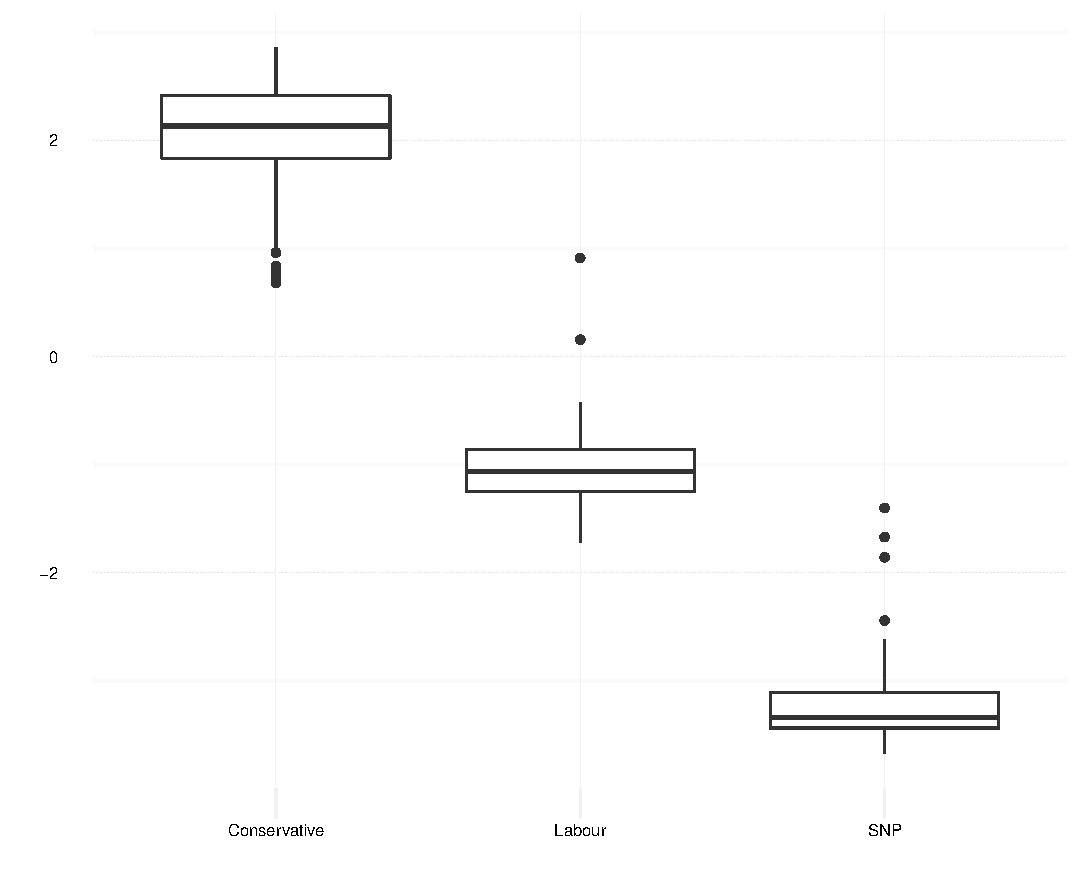
\includegraphics[scale=.75]{../figs/parl_box.pdf}
\label{fig:fig1}
\end{figure}

\subsection*{Measuring Ideology Using Speech}

To estimate a model of how speech relates to ideology, we use parliamentary speech as training data. Compared to the US, the UK has two major limitations. Firstly, because of whipping, votes by members of parliament do not convey much information beyond party affiliation. Thus, we can only learn about association between words and party. Secondly, the UK has multiple parties that cannot be cleanly aligned on the left-right axis. To account for that, we ignore speeches by members of any other party than Labour and Conservatives.

Our legislative speech data derive from two sources. First, we include 209,871 unique speeches by Labour and Conservative MPs from the period July 7, 2011 to March 11, 2014, available through the \textit{Digging into Linked Parliamentary Data} project \citep{marx2009advanced}.\footnote{Data are available from: \url{http://search.politicalmashup.nl/about.html}.} Not surprising, members of the Cabinet were frequent speakers, with Prime Minister David Cameron recording 5983 unique speeches. In contrast the leader of the Labour party, Ed Miliband, spoke in 914 instances. Second, like \citet{gentzkow2015measuring}, we collect Robert's Rules of Order \citep{henry2011robert}.

Our news corpora has over 7 million articles covering over 400 media sources between 2005 to 2015. We limit ourselves to news sources that publish in English, and for which we have more than 1000 transcripts since 2011. We further limit ourselves to data from 2010 and beyond from these sources. This leaves us with 2,742,735 transcripts from 255 sources. (See \ref{si_media_sum} for a complete list of media sources, the date ranges and number of transcripts per media source.)

We start with the standard text preprocessing stems of lemmatizing, removing `stop words', and punctuation, losing all words less than 2 characters long, and converting all the words to lower case. We further assume a 1-, 2- Markov model of language, storing just frequency of bigrams and trigrams and removing order information. Next, as a way to get rid of parliamentary language, we remove all bigrams and trigrams that are part of Robert's Rules of Order. Since we plan to use the data to predict ideology of the news data, we take an additional step of removing bi- and tri-grams that don't exist in our news database. (See \citet{gentzkow2010} and \citet{martin2014}, among others who have used similar assumptions in modeling similar text.)  Next, we split the data into a test-set (20\%) and a training-set (80\%). Using these bigrams and trigrams, we estimated a Elastic Net regression \citep{zou2005regularization}, cross-validating to tune the parameter ($\lambda$).

\begin{align}
   \hat{\beta} = \text{arg} \min_{\beta} \lvert\lvert y - X\beta \rvert\rvert^2 + \lambda_2 \lvert\beta\rvert^2 + \lambda_1 \lvert\beta\rvert
\end{align}

Using Elastic Net, we achieved an out-of-sample precision of .74 (see Table \ref{tab:text_validation}). The top 100 predictors of Labour and Conservative speech are listed in \ref{si_top100}.  

\let\center\empty
\let\endcenter\relax
\begin{center}
% latex table generated in R 3.3.1 by xtable 1.8-2 package
% Fri Aug 26 13:58:54 2016
\begin{table}[!htb]
\centering
\caption{Out-of-sample Performance of the model} 
\label{tab:text_validation}
\begin{tabular}{lllll}
  \hline
party & precision & recall & f1score & support \\ 
  \hline
Conservative & 0.74 & 0.74 & 0.74 & 1981 \\ 
  Labour & 0.74 & 0.74 & 0.74 & 2019 \\ 
   \hline
\end{tabular}
\end{table}

\end{center}
We used this trained model to predict the ideology of the news sources. 

\section*{Results}

We start by plotting social network based estimates of ideology of a few prominent news organizations (see Figure \ref{fig:fig2}). All the prominent outlets we plot lie between the party medians, those a majority are slightly closer to the Labour party's median than the Conservative party. The median of the social network based ideology estimates of all the media sources in our data is also closer to the Labour median than the Conservative median (see Figure \ref{fig:fig4}). The results are consistent with \citet{barbera2016}, who find that American media outlets tend to lean toward the Democratic Party. The ordering of the prominent media outlets, if not the location, is consistent with their reputation. For e.g., Guardian is the closest to Labour, and well left of \emph{The Daily Mail} or the \emph{The Express}. Scaling text data offers similar insights. Our text based estimates put Guardian to the left of \emph{The Daily Mail} or the \emph{The Express}. 
 
Next, we plotted accounts within various media companies (see Figure \ref{fig:fig3}). Like \citet{barbera2016}, we find intra-outlet ideological heterogeneity. However, it is more muted than the US, where the ideological spread is much bigger. In the UK data, as one can see, estimates are, for the most part, between -1 and 1 on the x-axis, right in the middle of the Labour and Conservative medians. Thus journalists (or other accounts) for our media outlets are not typically as conservative as the median Tory, nor as liberal as the median Labour Party member, or certainly the SNP median.  Based on the data, the \emph{Economist} offers the greatest ideological spread. 

\begin{figure}[!htbp]
\centering
\caption{Distribution of Journalist Ideology by Outlet}
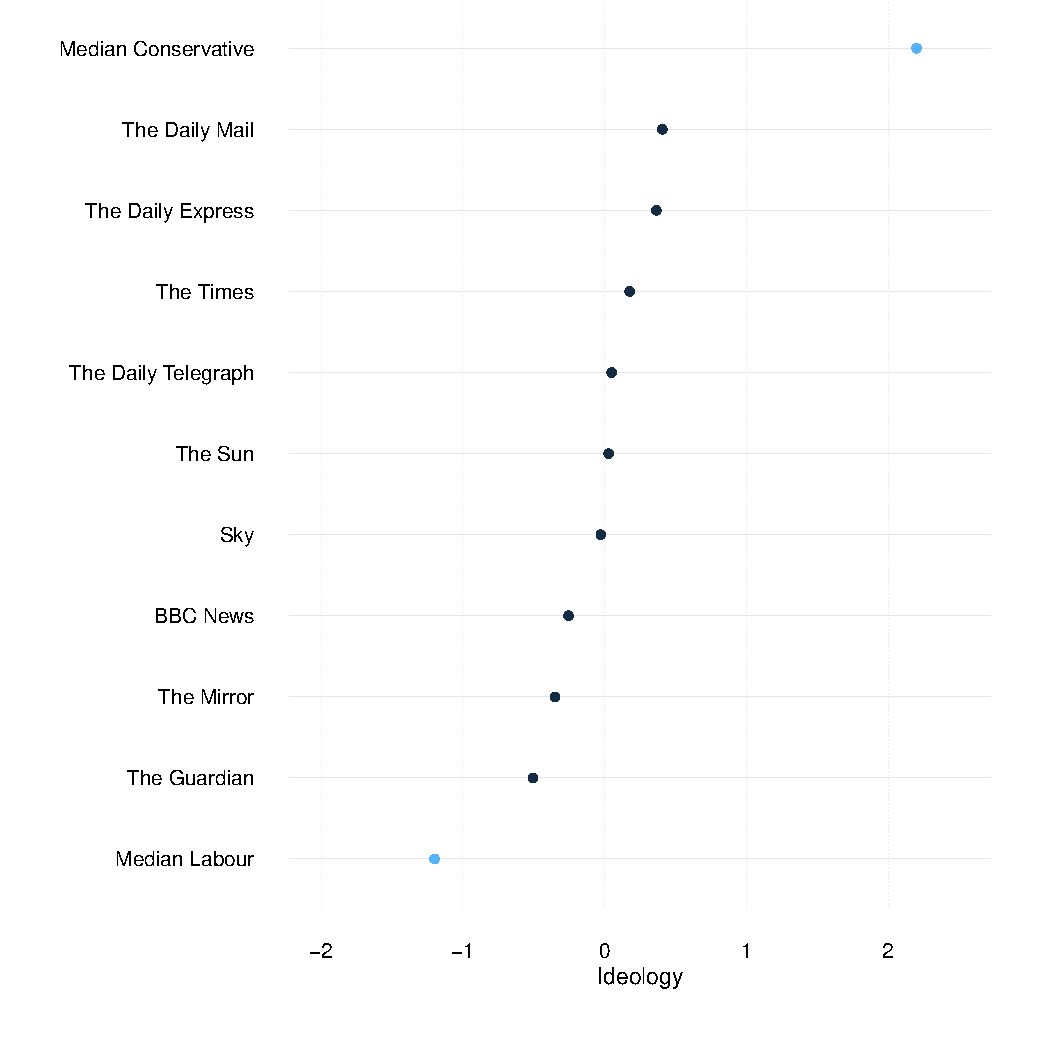
\includegraphics[scale=1]{../figs/line_plot_aug.pdf}
\label{fig:fig2}
\end{figure}

\begin{figure}[!htbp]
\centering
\caption{Distribution of Journalist Ideology by Outlet}
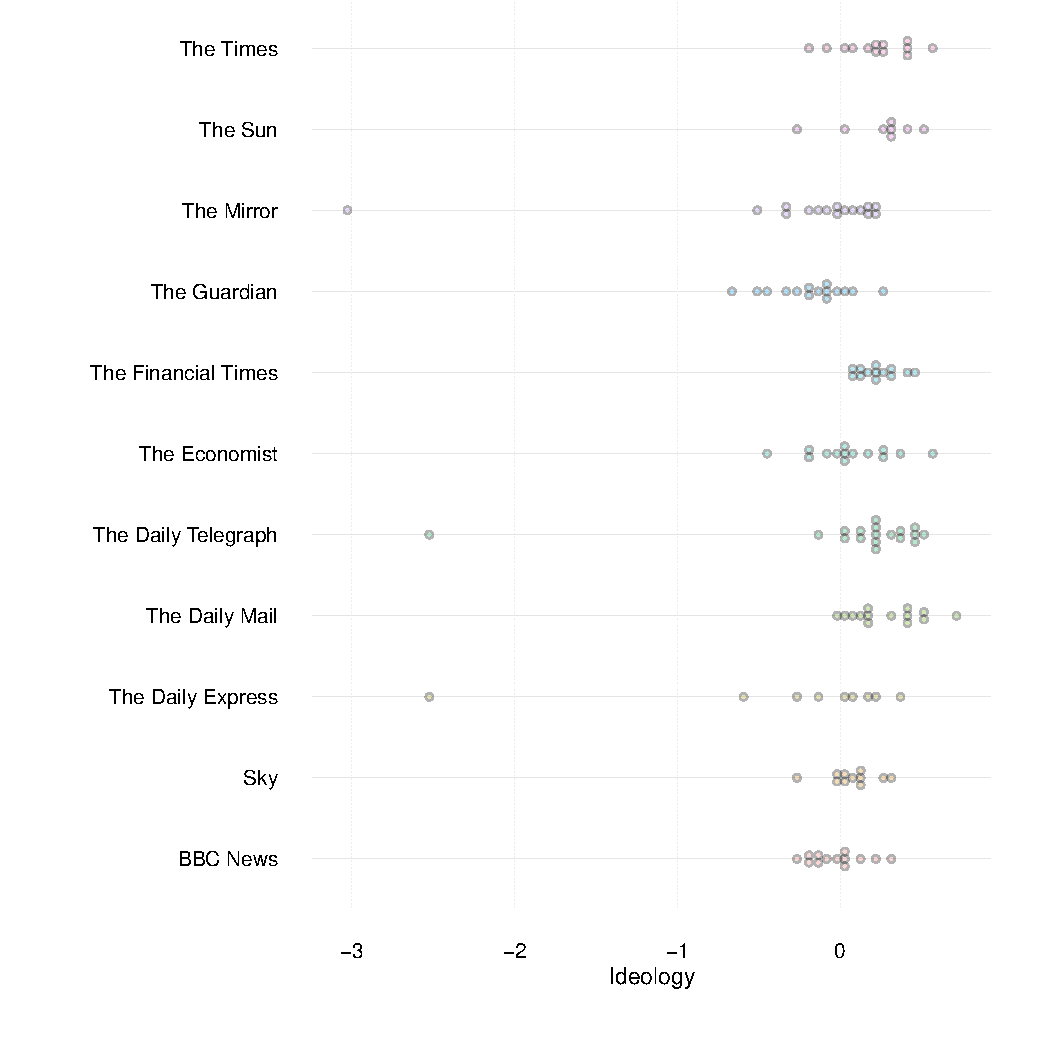
\includegraphics[scale=1]{../figs/media_dotplot_aug.pdf}
\label{fig:fig3}
\end{figure}


\section*{Discussion}

Accusations of news media bias are common. Some point to the fact that journalists tend to lean left, while others contend that publishers tend to be right-leaning. Still others note that both journalists and publishers may be able to distance themselves from their own views and ideas as they craft and distribute news content \citep[see][p. 250-258 for an overview]{morton2005}. Though, those working within media organizations note that editors and publishers exercise consideration discretion in determining what makes the news \citep{goldberg2001, orkent2004}.

These accusations are also concerning as research suggests a variety of consequences for biased news. For one, \citet{ladd2011} demonstrates that perceptions of media bias have been linked to a precipitous decline in media trust over time. Low levels of media trust have led citizens away from more balanced mainstream sources of news and into alternative and more partisan media, which has had consequences for citizens' political attitudes, beliefs, and voting behavior. Related, \citet{arceneaux2012} show that today's mainstream news environment presents oppositional voices sufficient to lead to polarization. Two, \citet{dellavigna2007} show that the expansion of Fox News---a source widely understood to favor conservative viewpoints---corresponded with an increase in the vote share for Republicans. Finally, returning to an older literature on the power of media endorsements of candidates in elections \citep[e.g][]{erikson1976}, \citet{ladd2009}, exploit a rare shift in editorial endorsement on the part of a leading newspaper in Britain show that the political voice of the media can have significant influence on its audience, with estimates of persuasion leading to vote change of the magnitude of 10 to 25 percent.

Methods of capturing bias, however, have been in want. Although in the past decade, scholars have turned to indirect measures based on either speech or social network data. The guiding principle for studies based on speech is that politicians communicate their left/right leanings in their statements made on the floor of the legislature. Media may also communicate their left/right leanings if they adopt similar ``speech" patterns to left/right politicians. Concerning the second approach, here the rationale is that social media users make informed decisions about who to follow. The aggregation of these informed decisions helps reveal information about the entity being followed. If a given news outlet is followed by members of the public who also follow liberal politicians, then we can infer that the outlet biases its information. Our approach has been to rely on both speech and social network data to present new estimates of media bias for the United Kingdom. Although our exercise has been a computationally intense one, our methodology is translatable to other Western democracies where the data exist.

\clearpage
\normalfont
\normalsize
\doublespace
\bibliographystyle{apsr}
\bibliography{multiple_measures}

\clearpage

\appendix
\renewcommand{\thesection}{SI \arabic{section}}
\renewcommand\thetable{\thesection.\arabic{table}}
\renewcommand\thefigure{\thesection.\arabic{figure}}
\counterwithin{figure}{section}

\begin{center}
\Large{Supporting Information}
\end{center}

\section{Distribution of Ideology of Media Sources}
\label{full_dist}
\begin{figure}[h]
\centering
\caption{Distribution of Social Network Based Estimates of Ideology of Media Sources}
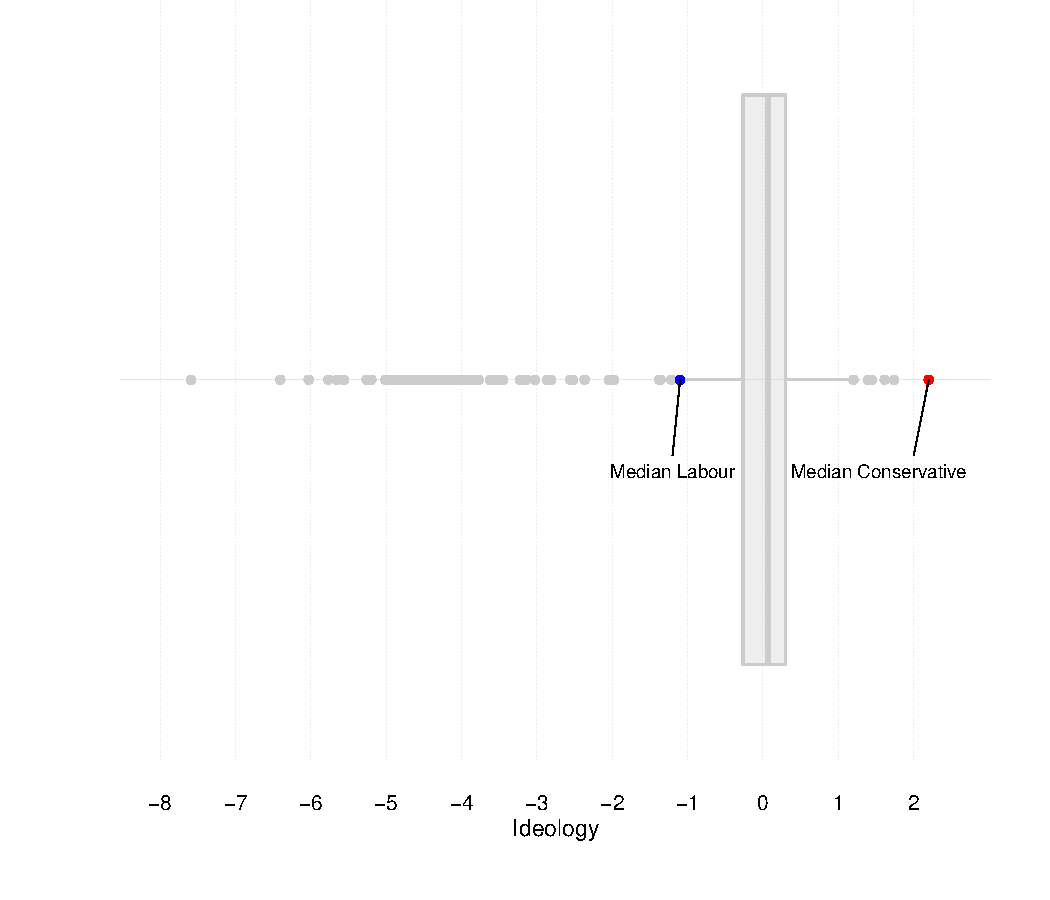
\includegraphics[scale=1]{../figs/boxplot_all_media_aug.pdf}
\label{fig:fig4}
\end{figure}

\clearpage

\label{full_dist}
\begin{figure}[h]
\centering
\caption{Distribution of Text Based Estimates of Ideology of Media Sources}
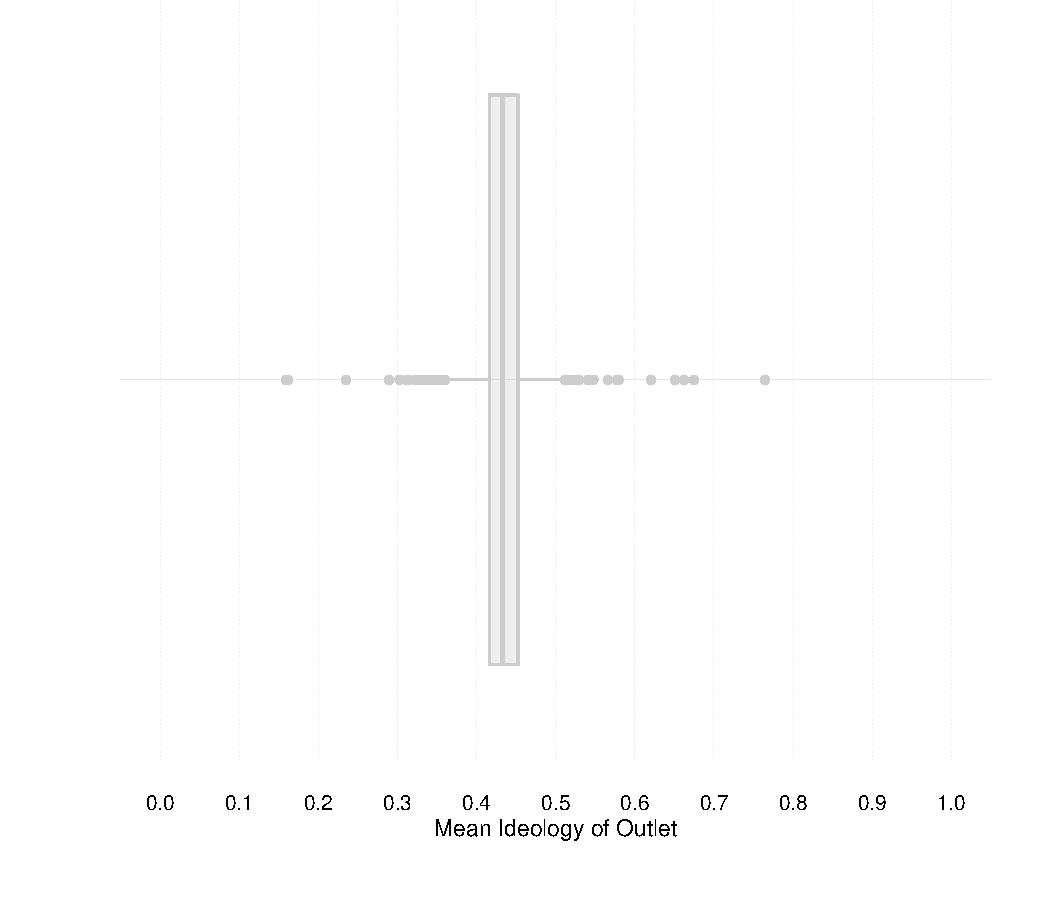
\includegraphics[scale=1]{../figs/hist_text_media.pdf}
\caption*{The x-axis maps proportion Conservative.}
\label{fig:fig5}
\end{figure}

\clearpage
\section{Top 100 Predictors of Labour and Conservative Speech}
\label{si_top100}
% latex table generated in R 3.3.1 by xtable 1.8-2 package
% Fri Aug 26 12:13:14 2016
\begingroup\scriptsize
\begin{longtable}{p{0.3\textwidth}p{0.3\textwidth}p{0.3\textwidth}}
\caption{Top 100 Predictors of Labour Speech} \\ 
  \hline
  \hline
friend home & also provid & social econom \\ 
  tori govern & vast major & ask whether \\ 
  tori parti & long overdu & intern commun \\ 
  trade union & futur job & inform avail \\ 
  opposit parti & later year & occupi territori \\ 
  busi secretari & wast manag & see benefit \\ 
  conserv parti & govern commit & east london \\ 
  govern member & welfar state & govern support \\ 
  south yorkshir & take forward & suppli chain \\ 
  previou administr & first time & want thank \\ 
  conserv member & follow consult & task forc \\ 
  point rais & winter fuel & play field \\ 
  bedroom tax & coal mine & direct travel \\ 
  work peopl & averag earn & militari action \\ 
  south wale & world bank & govern bodi \\ 
  greater manchest & daili mail & death penalti \\ 
  unit nation & missil defenc & said earlier \\ 
  new deal & public interest & state consid \\ 
  spend cut & transport system & conserv liber \\ 
  also ask & econom social & crime reduct \\ 
  labour govern & would inappropri & mani year \\ 
  much welcom & let say & receiv benefit \\ 
  good practic & govern open & school meal \\ 
  lib dem & job growth & plan growth \\ 
  way forward & bank levi & new member \\ 
  next week & hope right & chang cours \\ 
  work togeth & hunt dog & voluntari sector \\ 
  tax cut & committe agre & chief inspector \\ 
  poll tax & food bank & want take \\ 
  manifesto commit & invest public & social justic \\ 
  meet need & ensur peopl & year conserv \\ 
  doubledip recess & integr transport & energi compani \\ 
  local govern & tower hamlet &  \\ 
  peopl work & major chang &  \\ 
   \hline
\hline
\label{tab:top_100c}
\end{longtable}
\endgroup

\clearpage
% latex table generated in R 3.3.1 by xtable 1.8-2 package
% Fri Aug 26 12:13:14 2016
\begingroup\scriptsize
\begin{longtable}{p{0.3\textwidth}p{0.3\textwidth}p{0.3\textwidth}}
\caption{Top 100 Predictors of Conservative Speech} \\ 
  \hline
  \hline
labour member & govern fail & point view \\ 
  offici report & prime minist & meet target \\ 
  minist may & minist give & state govern \\ 
  secretari state & statement hous & counti council \\ 
  financi secretari & govern think & interest hear \\ 
  minist said & anoth exampl & govern account \\ 
  labour parti & minist state & statut book \\ 
  agre hous & grammar school & much hope \\ 
  minist would & south west & urg minist \\ 
  declar interest & govern claim & hope govern \\ 
  govern seem & move hous & huge amount \\ 
  good point & one thing & govern target \\ 
  side hous & govern seek & high speed \\ 
  coalit govern & home secretari & difficult time \\ 
  polit correct & yet anoth & almost everi \\ 
  tell us & budget deficit & conserv believ \\ 
  public financ & none less & per annum \\ 
  great pleasur & increas cost & get wors \\ 
  may well & town centr & rule law \\ 
  fact govern & person account & lord mandelson \\ 
  red tape & district council & press releas \\ 
  would like & minist say & mental ill \\ 
  govern intend & govern failur & minist make \\ 
  last govern & pupil premium & spend much \\ 
  european court & quit lot & boundari commiss \\ 
  minist confirm & said govern & lucki enough \\ 
  new labour & reform public & one two \\ 
  minist agre & govern tri & green deal \\ 
  govern may & absolut right & cold war \\ 
  would enabl & hold govern & govern one \\ 
  would grate & margaret thatcher & special educ \\ 
  hous built & one could & shadow minist \\ 
  nation interest & fuel duti &  \\ 
  govern say & govern want &  \\ 
   \hline
\hline
\label{tab:top_100c}
\end{longtable}
\endgroup

\clearpage

\section{Summary of the Media Data}
\label{si_media_sum}
% latex table generated in R 3.3.1 by xtable 1.8-2 package
% Fri Aug 26 12:13:14 2016
\begingroup\tiny
\begin{longtable}{p{0.3\textwidth}p{0.1\textwidth}p{0.15\textwidth}p{0.15\textwidth}}
\caption{Summary of the Media Data} \\ 
  \hline
Name & No. of Transcripts & From & To \\ 
  \hline
24dash & 17207 & 2010-01-04 & 2012-04-16 \\ 
  a World to Win Blogs & 1550 & 2012-01-06 & 2014-09-29 \\ 
  Agra-Net.com & 14322 & 2010-07-28 & 2014-03-21 \\ 
  Alert Net & 15154 & 2010-09-01 & 2013-04-23 \\ 
  Alliance for Workers' Liberty & 1646 & 2010-06-16 & 2014-07-08 \\ 
  Ananova & 24495 & 2010-01-01 & 2011-11-21 \\ 
  Ananova - Orange News & 8003 & 2010-03-20 & 2012-09-24 \\ 
  Andover Advertiser & 3666 & 2010-01-01 & 2014-08-25 \\ 
  Asharq Al-Awsat & 19107 & 2010-01-01 & 2013-02-26 \\ 
  Ayrshire Post & 5639 & 2011-12-29 & 2013-06-30 \\ 
  Bakery and Snacks & 2549 & 2010-01-01 & 2013-01-14 \\ 
  Ballyclare Gazette & 1029 & 2010-01-04 & 2014-01-16 \\ 
  Ballymena Today & 1327 & 2010-01-05 & 2011-12-05 \\ 
  Ballymoney Today & 20310 & 2010-01-04 & 2011-02-09 \\ 
  Banbridge Leader & 1256 & 2011-10-28 & 2012-07-05 \\ 
  Banbridge Today & 28471 & 2010-01-01 & 2011-10-31 \\ 
  Banbury Guardian & 17762 & 2010-01-01 & 2013-06-27 \\ 
  Barking and Dagenham Post & 1160 & 2010-01-04 & 2010-09-23 \\ 
  Barnesley Chronicle & 1575 & 2010-01-05 & 2011-12-06 \\ 
  Barnet Times & 28793 & 2010-01-01 & 2011-12-13 \\ 
  Basingstoke Gazette & 14265 & 2010-01-01 & 2014-07-12 \\ 
  Bbc - Leicester News & 2093 & 2010-01-01 & 2012-04-11 \\ 
  Bbc News - Uk & 2257 & 2012-04-18 & 2015-02-04 \\ 
  Bbc News Europe & 79632 & 2010-07-15 & 2015-02-04 \\ 
  Beccles and Bungay Journal & 1745 & 2010-01-02 & 2010-09-27 \\ 
  Bedford Times and Citizen & 6884 & 2010-01-01 & 2011-11-07 \\ 
  Bedford Today & 2484 & 2011-11-07 & 2013-06-28 \\ 
  Belfast Media & 4475 & 2010-01-04 & 2011-09-15 \\ 
  Belfast Telegraph & 154231 & 2010-01-01 & 2013-06-04 \\ 
  Belfast Today & 1948 & 2012-01-01 & 2012-07-04 \\ 
  Berwick Today & 2099 & 2010-01-04 & 2011-12-12 \\ 
  Bexhill Observer & 3191 & 2010-01-01 & 2013-06-22 \\ 
  Bexhill Today & 1900 & 2010-01-01 & 2011-12-05 \\ 
  Birmingham Mail & 66692 & 2010-01-01 & 2014-07-08 \\ 
  Bishop's Stortford Citizen & 50449 & 2010-01-01 & 2012-08-31 \\ 
  Blackburn Citizen & 13311 & 2010-01-01 & 2014-05-23 \\ 
  Blackpool Today & 3249 & 2010-01-01 & 2011-01-12 \\ 
  Bognor Regis Observer & 2936 & 2011-12-07 & 2015-02-04 \\ 
  Bognor Today & 5956 & 2010-01-01 & 2011-12-13 \\ 
  Bolton News & 56276 & 2010-01-01 & 2013-06-30 \\ 
  Borehamwood and Elstree Times & 61627 & 2010-01-01 & 2014-07-08 \\ 
  Boston Standard & 1402 & 2011-12-13 & 2012-07-04 \\ 
  Boston Today & 2215 & 2010-01-04 & 2011-12-13 \\ 
  Bracknell Forest Standard & 4804 & 2010-01-22 & 2013-06-11 \\ 
  Bradford Telegraph and Argus & 15179 & 2012-01-03 & 2014-05-23 \\ 
  Brechin Today & 17536 & 2010-01-06 & 2011-12-11 \\ 
  Brighton Evening Argus & 9113 & 2010-05-01 & 2014-09-06 \\ 
  Buckingham Today & 37900 & 2010-01-01 & 2011-12-01 \\ 
  Bucks Free Press & 6196 & 2012-01-01 & 2014-07-08 \\ 
  Bucks Herald & 5101 & 2010-01-04 & 2013-06-27 \\ 
  Burnley Express & 1119 & 2011-12-07 & 2012-07-03 \\ 
  Burnley Today & 4692 & 2010-01-03 & 2011-12-07 \\ 
  Bury Free Press & 3112 & 2011-11-25 & 2013-06-24 \\ 
  Bury St Edmunds Today & 5253 & 2010-01-01 & 2011-12-15 \\ 
  Bury Times & 4545 & 2010-01-01 & 2014-07-12 \\ 
  Buxton Advertiser & 31293 & 2010-01-01 & 2012-07-03 \\ 
  Cambridge Evening News & 7232 & 2010-01-01 & 2011-10-27 \\ 
  Cambridge News & 2047 & 2011-10-27 & 2012-09-17 \\ 
  Cambs Times & 9804 & 2010-01-01 & 2014-07-08 \\ 
  Chard and Ilminster News & 9213 & 2010-01-01 & 2014-05-23 \\ 
  Cheshire Online & 10284 & 2012-01-01 & 2013-06-27 \\ 
  Chester Evening Leader & 2785 & 2010-01-04 & 2011-12-13 \\ 
  Chester First & 1197 & 2011-12-06 & 2013-06-13 \\ 
  Chester Standard & 3534 & 2010-01-03 & 2011-12-05 \\ 
  Chester Standard and Leader & 1391 & 2011-12-12 & 2013-06-20 \\ 
  Chichester Observer & 8224 & 2010-01-01 & 2012-07-05 \\ 
  Chingford Guardian & 11802 & 2010-01-01 & 2014-08-25 \\ 
  Chorley Citizen & 4880 & 2010-01-01 & 2014-07-07 \\ 
  Clitheroe Today & 1719 & 2010-01-01 & 2011-02-16 \\ 
  Colchester Daily Gazette & 14218 & 2012-01-01 & 2015-02-04 \\ 
  Cornish Guardian & 16969 & 2010-12-15 & 2014-03-18 \\ 
  Country Life & 1730 & 2010-01-04 & 2012-03-26 \\ 
  Coventry Telegraph & 6842 & 2012-01-01 & 2013-06-27 \\ 
  Crawley Observer & 7371 & 2010-01-01 & 2013-06-27 \\ 
  Croydon Guardian & 13676 & 2010-01-01 & 2014-08-25 \\ 
  Cumberland and Westmorland Herald & 1238 & 2010-01-04 & 2013-06-27 \\ 
  Daily Express & 4220 & 2010-01-01 & 2013-02-06 \\ 
  Daily Post & 16752 & 2012-01-01 & 2015-02-04 \\ 
  Daily Record & 12067 & 2011-12-31 & 2012-07-31 \\ 
  Darlington and Stockton Times & 12830 & 2011-12-29 & 2014-05-23 \\ 
  Derby Evening Telegraph & 21616 & 2011-12-30 & 2013-08-31 \\ 
  Derbyshire Times & 1455 & 2012-01-01 & 2012-07-04 \\ 
  Derry Journal & 2680 & 2012-01-01 & 2013-06-22 \\ 
  Diss Mercury & 1771 & 2012-01-01 & 2014-10-09 \\ 
  Doncaster Free Press & 2260 & 2011-12-30 & 2012-07-02 \\ 
  Dorset Daily Echo & 7353 & 2011-12-30 & 2014-04-02 \\ 
  Driffield Times and Post & 1003 & 2011-12-29 & 2013-07-01 \\ 
  Dunmow Broadcast & 1237 & 2012-04-03 & 2014-11-11 \\ 
  East Lothian Courier & 2745 & 2011-07-15 & 2014-04-02 \\ 
  Eastern Daily Press & 20077 & 2011-12-30 & 2014-07-08 \\ 
  Eastwood Advertiser & 1254 & 2011-12-28 & 2013-06-30 \\ 
  Echo - Essex News and Sports & 8099 & 2011-10-22 & 2014-08-25 \\ 
  Edgware and Mill Hill Times & 3218 & 2012-01-02 & 2012-08-31 \\ 
  Ely Standard & 3444 & 2012-01-02 & 2014-11-12 \\ 
  Epsom Guardian & 5439 & 2010-02-09 & 2014-05-22 \\ 
  Essex Chronicle & 6514 & 2012-01-01 & 2013-12-11 \\ 
  Eubusiness & 6510 & 2012-01-01 & 2014-07-08 \\ 
  Evening Star (Ipswich) & 10214 & 2012-01-01 & 2015-02-04 \\ 
  Express and Star & 6866 & 2012-01-02 & 2015-02-04 \\ 
  Farmer's Weekly Special Reports & 2449 & 2011-12-29 & 2012-08-30 \\ 
  Farmers Guardian & 5873 & 2011-03-03 & 2015-02-04 \\ 
  Farmers Weekly Interactive & 5914 & 2011-12-30 & 2014-07-04 \\ 
  Farming Uk & 3382 & 2012-01-01 & 2014-12-11 \\ 
  Food Navigator & 3395 & 2012-01-02 & 2015-02-04 \\ 
  Food Quality News & 1612 & 2012-01-02 & 2015-02-03 \\ 
  Fruit Net (Uk and Germany) & 1576 & 2012-01-03 & 2012-10-24 \\ 
  Gazette and Herald & 7376 & 2012-01-03 & 2014-05-23 \\ 
  Gazette Live & 12090 & 2010-04-10 & 2013-04-29 \\ 
  Glasgow Evening Times & 4013 & 2011-12-30 & 2013-06-27 \\ 
  Grantham Today & 3049 & 2012-01-01 & 2013-06-18 \\ 
  Grimsby Telegraph & 3332 & 2012-01-01 & 2013-08-31 \\ 
  Guardian Local & 2860 & 2010-03-26 & 2014-01-10 \\ 
  Guardian Series & 5601 & 2011-12-31 & 2014-08-25 \\ 
  Hampshire Chronicle & 3635 & 2012-01-01 & 2014-07-08 \\ 
  Harborough Mail & 1639 & 2012-01-02 & 2013-08-01 \\ 
  Haringey Independent & 2970 & 2012-01-01 & 2012-08-31 \\ 
  Harlow Citizen and Guardian & 3006 & 2012-01-04 & 2014-08-25 \\ 
  Harrow Times & 5262 & 2010-01-04 & 2014-07-08 \\ 
  Hartle Pool Mail & 18306 & 2010-01-05 & 2013-05-21 \\ 
  Hemel Hempstead Today & 3693 & 2012-01-01 & 2013-06-19 \\ 
  Hendon and Finchley, Barnet and Potters Bar, and Edgeware and Mills Hill Times & 3115 & 2010-01-06 & 2014-05-23 \\ 
  Herald Scotland Breaking News & 22100 & 2011-12-31 & 2015-02-04 \\ 
  Herts and Essex Observer & 3302 & 2012-01-02 & 2014-07-08 \\ 
  Hexham Courant & 1259 & 2012-01-02 & 2015-02-03 \\ 
  Highland News & 1054 & 2012-01-02 & 2014-05-22 \\ 
  Horncastle News & 1231 & 2010-07-07 & 2013-08-30 \\ 
  Horticulture Week & 1281 & 2012-01-03 & 2012-10-23 \\ 
  Hucknall Dispatch & 1712 & 2012-01-01 & 2013-08-31 \\ 
  Hull Daily Mail & 18491 & 2012-01-02 & 2013-08-30 \\ 
  Hunts Post & 2484 & 2011-12-30 & 2014-11-25 \\ 
  Ic Newcastle & 1989 & 2011-12-27 & 2013-02-12 \\ 
  Ilford Recorder & 2092 & 2010-01-01 & 2014-10-27 \\ 
  Ilkeston Advertiser & 2619 & 2011-12-05 & 2013-08-31 \\ 
  Ilkley Gazette & 2206 & 2012-01-01 & 2012-08-31 \\ 
  Impartial Reporter & 1981 & 2011-12-29 & 2013-01-09 \\ 
  Insurance Insight & 1565 & 2012-03-30 & 2013-12-09 \\ 
  International Business Times & 8819 & 2012-01-01 & 2012-04-25 \\ 
  International Business Times Uk & 37441 & 2012-04-24 & 2015-02-04 \\ 
  Isle of Wight County Press & 5592 & 2012-01-01 & 2014-09-14 \\ 
  Journal Live & 8775 & 2012-01-01 & 2013-06-27 \\ 
  Kenilworth Weekly News & 1148 & 2012-01-01 & 2013-08-07 \\ 
  Kingston Guardian & 5569 & 2010-02-09 & 2014-08-25 \\ 
  Lancashire Evening Post & 12836 & 2011-12-27 & 2014-04-02 \\ 
  Lancashire Evening Telegraph & 7987 & 2010-07-09 & 2014-05-03 \\ 
  Lancashire Telegraph & 14232 & 2010-01-06 & 2014-07-08 \\ 
  Leamington Observer & 1504 & 2012-11-23 & 2015-02-04 \\ 
  Leicester Mercury & 19822 & 2012-01-01 & 2013-09-01 \\ 
  Leigh Journal & 4266 & 2010-06-16 & 2014-08-25 \\ 
  Lincolnshire Echo & 11841 & 2012-01-01 & 2013-12-17 \\ 
  Liverpool Echo & 31745 & 2010-10-25 & 2013-03-11 \\ 
  Local London & 13308 & 2010-05-09 & 2014-07-12 \\ 
  Louth Leader & 2459 & 2011-12-05 & 2013-08-09 \\ 
  Lurgan Mail & 3717 & 2010-02-18 & 2013-08-30 \\ 
  Luton News Herald and Post & 1529 & 2012-01-01 & 2012-07-04 \\ 
  Lynn News & 2400 & 2012-01-01 & 2012-07-04 \\ 
  Manchester Online & 12576 & 2010-04-19 & 2013-01-23 \\ 
  Mansfield and Ashfield Chad & 3631 & 2011-12-15 & 2015-01-27 \\ 
  Matlock Mercury & 2387 & 2011-12-29 & 2013-08-30 \\ 
  Meat Info & 2170 & 2012-01-03 & 2015-02-04 \\ 
  Melton Times & 4016 & 2011-12-27 & 2013-12-13 \\ 
  Metro & 14411 & 2012-01-01 & 2015-02-04 \\ 
  Morning Star & 7287 & 2012-01-01 & 2013-06-30 \\ 
  Morning Star Online & 1368 & 2013-05-23 & 2013-08-29 \\ 
  Morpeth Herald & 2510 & 2012-01-01 & 2013-08-05 \\ 
  Newbury Today & 5100 & 2010-01-12 & 2014-09-15 \\ 
  Newham Recorder & 3799 & 2012-01-03 & 2014-10-27 \\ 
  News and Star & 3229 & 2011-12-27 & 2013-07-31 \\ 
  News Guardian & 1783 & 2012-01-02 & 2013-06-27 \\ 
  News Post Leader & 4272 & 2010-01-04 & 2013-06-29 \\ 
  News Shopper & 5921 & 2011-12-27 & 2014-07-08 \\ 
  Newsnet Scotland & 5266 & 2011-07-22 & 2014-12-10 \\ 
  North Wales Chronicle & 1821 & 2010-01-18 & 2014-09-15 \\ 
  North-West Evening Mail & 5649 & 2011-12-31 & 2015-02-03 \\ 
  Northampton Chronicle and Echo & 13018 & 2012-01-01 & 2015-02-04 \\ 
  Northamptonshire Evening Telegraph & 2059 & 2012-01-01 & 2012-05-30 \\ 
  Northern Ireland Executive & 5634 & 2012-01-11 & 2015-02-04 \\ 
  Northumberland Gazette & 1781 & 2011-12-29 & 2013-08-04 \\ 
  Norwich Evening News 24 & 16705 & 2011-09-07 & 2015-02-04 \\ 
  Nottingham Post & 23001 & 2012-01-01 & 2013-08-31 \\ 
  Open Democracy & 1024 & 2011-01-28 & 2012-06-25 \\ 
  Ormskirk and Skelmersdale Advertiser & 4601 & 2012-01-03 & 2014-03-26 \\ 
  Oxford Mail & 47233 & 2012-01-01 & 2015-02-04 \\ 
  Paisley Daily Express & 4608 & 2011-12-30 & 2012-12-18 \\ 
  Peterborough Evening Telegraph & 10155 & 2011-12-30 & 2013-05-09 \\ 
  Petersfield Post & 5331 & 2010-01-07 & 2014-01-24 \\ 
  Pink News & 4564 & 2012-01-03 & 2013-08-30 \\ 
  Plymouth Herald & 3350 & 2012-06-07 & 2013-08-31 \\ 
  Pr Newswire & 4146 & 2011-12-30 & 2013-08-13 \\ 
  Reading Post & 7965 & 2012-01-03 & 2015-02-03 \\ 
  Redhill and Reigate Life & 2082 & 2012-01-01 & 2015-01-27 \\ 
  Retford Trader and Guardian & 3688 & 2012-01-01 & 2013-08-31 \\ 
  Reuters Alertnet & 19103 & 2010-01-01 & 2012-10-19 \\ 
  Richmond and Twickenham Times & 3149 & 2011-12-31 & 2014-08-25 \\ 
  Ripley and Heanor News & 2679 & 2011-12-30 & 2013-08-30 \\ 
  Royston Crow & 3899 & 2012-01-03 & 2015-02-03 \\ 
  Rutland Times & 6112 & 2011-12-08 & 2013-08-26 \\ 
  Rye and Battle Observer & 1276 & 2011-12-30 & 2013-06-25 \\ 
  Saffron Walden Reporter & 2870 & 2011-12-27 & 2014-11-11 \\ 
  Sale and Altrincham Messenger & 3659 & 2012-01-01 & 2014-05-23 \\ 
  Scunthorpe Telegraph & 9198 & 2012-01-01 & 2013-08-31 \\ 
  Sheffield Today & 6284 & 2012-01-01 & 2012-07-04 \\ 
  Skynews & 16526 & 2011-12-30 & 2014-05-23 \\ 
  Slough and South Bucks Observer & 2514 & 2012-01-01 & 2013-06-30 \\ 
  Somerset County Gazette & 5017 & 2012-01-01 & 2014-09-09 \\ 
  South Wales Evening Post & 11987 & 2013-01-01 & 2015-02-04 \\ 
  Southern Daily Echo & 41764 & 2010-01-01 & 2012-08-31 \\ 
  Southern Daily Echo - this is Hampshire & 8250 & 2010-02-09 & 2014-09-12 \\ 
  Spalding Guardian & 4331 & 2011-12-11 & 2013-06-20 \\ 
  Stamford Mercury & 1585 & 2012-01-01 & 2012-07-04 \\ 
  Streatham Guardian & 1317 & 2010-05-10 & 2012-02-21 \\ 
  Sunderland Echo & 2900 & 2012-01-01 & 2012-07-03 \\ 
  Surrey Advertiser & 4406 & 2010-01-05 & 2013-01-11 \\ 
  Sutton Guardian & 4483 & 2012-01-01 & 2014-07-08 \\ 
  Telegraph Uk & 5398 & 2011-12-30 & 2013-11-05 \\ 
  The Bath Chronicle & 10460 & 2012-01-01 & 2013-09-02 \\ 
  The Berwickshire News & 14351 & 2010-01-02 & 2013-06-27 \\ 
  The Courier and Advertiser & 2646 & 2012-01-02 & 2012-12-11 \\ 
  The Cumberland News & 15602 & 2010-01-01 & 2015-01-30 \\ 
  The Daily Mail & 138438 & 2010-11-01 & 2014-05-23 \\ 
  The Daily Star & 21226 & 2010-04-01 & 2013-07-01 \\ 
  The Daily Telegraph & 284107 & 2010-01-01 & 2015-02-04 \\ 
  The Farmers Guardian & 1726 & 2010-04-26 & 2012-10-03 \\ 
  The Guardian & 9457 & 2011-12-28 & 2014-10-27 \\ 
  The Guardian Europe & 17262 & 2012-05-09 & 2014-09-15 \\ 
  The Guardian Uk & 2230 & 2011-07-19 & 2013-07-01 \\ 
  The Herald (Scotland) & 15984 & 2012-02-05 & 2014-09-15 \\ 
  The Independent Uk & 16763 & 2012-02-09 & 2013-06-30 \\ 
  The Northern Echo & 8602 & 2011-12-31 & 2012-08-30 \\ 
  The Pig Site - Uk & 1079 & 2011-12-29 & 2012-05-11 \\ 
  The Press (York) & 14108 & 2010-01-04 & 2014-04-01 \\ 
  The Press and Journal & 4970 & 2012-01-02 & 2014-05-21 \\ 
  The Reading Chronicle & 4771 & 2012-01-01 & 2013-01-09 \\ 
  The Scotsman & 25747 & 2012-02-08 & 2013-07-01 \\ 
  this is Cheshire & 4804 & 2012-01-01 & 2014-09-04 \\ 
  this is Exeter & 14939 & 2012-01-02 & 2013-08-30 \\ 
  this is Gloucestershire & 28894 & 2011-12-31 & 2013-12-05 \\ 
  Times and Star & 1553 & 2011-12-23 & 2015-02-03 \\ 
  Tyrone Times & 3679 & 2012-04-11 & 2013-08-30 \\ 
  Uk Uncut on Twitter & 2492 & 2012-01-04 & 2012-05-23 \\ 
  Waltham Forest Guardian & 6406 & 2012-01-01 & 2014-08-25 \\ 
  Wandsworth Guardian & 8654 & 2012-01-01 & 2012-08-31 \\ 
  Wanstead and Woodford Guardian & 1099 & 2012-01-01 & 2012-08-28 \\ 
  West Sussex County Times & 3426 & 2012-01-01 & 2013-06-10 \\ 
  Western Mail & 6319 & 2011-04-08 & 2013-04-09 \\ 
  Wharf & 3249 & 2012-01-03 & 2015-02-05 \\ 
  Wiltshire News / this is Wiltshire & 16539 & 2012-01-02 & 2015-02-04 \\ 
  Wirral Globe & 2466 & 2012-01-01 & 2014-08-25 \\ 
  Wisbech Standard & 5109 & 2011-12-30 & 2014-11-19 \\ 
  Wokingham Times & 5488 & 2010-01-26 & 2013-06-10 \\ 
  Worcester News & 9961 & 2012-01-01 & 2014-07-08 \\ 
  Worksop Guardian & 3851 & 2011-12-28 & 2013-08-23 \\ 
  World Nuclear News & 1041 & 2012-01-03 & 2014-08-27 \\ 
  Worthing Herald & 3096 & 2011-12-06 & 2015-02-04 \\ 
  Yorkshire Evening Post & 19816 & 2011-08-23 & 2013-06-06 \\ 
  Yorkshire Post & 1012 & 2013-01-15 & 2013-06-05 \\ 
   \hline
\hline
\label{tab:summary}
\end{longtable}
\endgroup


\end{document} 